\documentclass{article}

\usepackage{lipsum}
\usepackage{color}
\usepackage{amsmath}
\usepackage{graphicx}
\usepackage{float}


\title {CSE300\textunderscore Assignment1\\Introduction to\LaTeX\\Albert Einstein}
\author{Subangkar Karmaker Shanto\\Student ID: 1505015}

\date{}

\begin{document}
\begin{titlepage}
\maketitle
\thispagestyle{empty}
\null
\vfill
\begin{figure}[h]
    \centering
    
\includegraphics[width=.25\textwidth]{figures/logoBIRN.png}
    \label{fig:logo}
\end{figure}
\begin{center}
Department of Computer Science and Engineering \\Bangladesh University of Engineering and Technology\\(BUET)\\Dhaka 1000 \\
\date{\today}
    
\end{center}
\end{titlepage}

\newpage


\section{Introduction}



\begin{figure}[h!]
    % \centering
    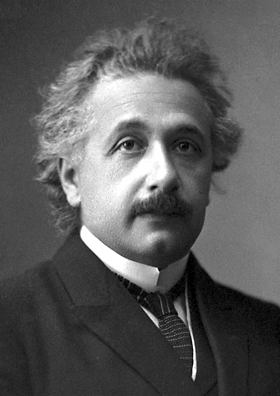
\includegraphics[width=10cm,height=6cm,keepaspectratio]{figures/Albert_Einstein_(Nobel).png}
    % \caption{Albert_Einstein}
    \label{fig:einstein_ProPic}
\end{figure}

Albert Einstein (14 March 1879 – 18 April 1955) was a German-born theoretical physicist who developed the theory of relativity, one of the two pillars of modern physics (alongside quantum mechanics). His work is also known for its influence on the philosophy of science.He is best known by the general public for his mass–energy equivalence formula \textbf{$E = mc^2$} (which has been dubbed \textbf{\textit{"the world's most famous equation"}}).He received the \textbf{1921 Nobel Prize in Physics} \textit{"for his services to theoretical physics, and especially for his discovery of the law of the photoelectric effect"}, a pivotal step in the evolution of quantum theory.






\end{document}